\documentclass[conference]{IEEEtran}

\usepackage[utf8]{inputenc}
\usepackage[T1]{fontenc}
\usepackage[czech]{babel}
\usepackage{cite}
\usepackage{amsmath,amssymb,amsfonts}
\usepackage{booktabs}
\usepackage{graphicx}
\usepackage{textcomp}
\usepackage{xcolor}
\usepackage{url}

\newcommand{\code}[1]{\texttt{#1}}
\newcommand{\placeholder}[1]{%
  \fbox{%
    \begin{minipage}{0.92\linewidth}
      \centering\small #1
    \end{minipage}%
  }%
}

\begin{document}

\title{FxLMS algoritmus pro potlačení zvukové stopy dronu pro účely detekce akustických impulzních událostí}

\author{\IEEEauthorblockN{Martin Maxa}
\IEEEauthorblockA{CTU, FEE\\
Prague, Czechia\\
maxamart@fel.cvut.cz}}

\maketitle

\begin{abstract}
Palubní mikrofon dronu měří kromě okolních událostí i vlastní hluk motorů a vrtulí. U krátkých impulzních signálů, například výstřelu, může tato složka zhoršit poměr signálu k rušení natolik, že jednoduchý detektor pracuje s nespolehlivým vstupem. Tento text navrhuje a popisuje simulovanou implementaci aktivního potlačení hluku založenou na algoritmu filtered-x least mean square (FxLMS). Referenční vstupy jsou odvozeny přímo z~řídicích signálů motorů, bez použití referenčních mikrofonů, a~adaptivní filtr minimalizuje reziduální hluk v~chybovém mikrofonním signálu. Adaptace používá normalizovaný (NLMS) krok, jehož efektivní velikost je dělena okamžitým výkonem filtrované reference sečteným přes všechny kanály; tím je stejná rychlost učení stabilní pro SISO i~vícekanálové konfigurace bez ručního ladění. Text uvádí rovnice FxLMS, převod algoritmu do Q15 fixed-point C kódu a metodiku pro SISO, sum-first a MISO režimy. Kvantitativní výsledky budou doplněny po finálním vygenerování grafů a metrik.
\end{abstract}

\begin{IEEEkeywords}
active noise control, FxLMS, adaptive filtering, drone acoustics, impulsní akustické události
\end{IEEEkeywords}

\section{Úvod}
Dron vytváří výraznou periodickou akustickou složku na blade pass frequency (BPF), tedy frekvenci průchodu listů vrtule. Pro vrtuli s~$N_b$ listy a~otáčkovou frekvencí $f_r$ platí $f_{\mathrm{BPF}}=N_b f_r$; ve spektru se kromě základní BPF objevují také její harmonické. Právě tato tonální maxima tvoří hlavní pozorovanou strukturu dronového hluku a~leží převážně pod 1\,kHz, jak ukazuje obr.~\ref{fig:dads_spectrum}. Palubní mikrofon proto kromě okolních událostí zaznamenává i~vlastní pohon; u~krátkých impulzních událostí může tato složka zhoršit poměr signálu k~rušení.

Aktivní potlačení hluku (ANC) používá řízený sekundární zdroj zvuku a snaží se v chybovém místě snížit akustický tlak rušení \cite{elliott1993active,kuo1996anc}. Feedforward varianta potřebuje referenci korelovanou s rušením. V~navrženém systému ji nezískáváme z~referenčních mikrofonů, ale přímo z~řídicích signálů jednotlivých motorů, z~nichž lze odvodit okamžitou BPF. Základní LMS však pro ANC nestačí, protože odrušovací signál se do chybového mikrofonu dostane přes sekundární akustickou cestu. Algoritmus filtered-x LMS (FxLMS) proto v adaptační větvi používá referenci filtrovanou odhadem této cesty \cite{burgess1981duct,widrow1985adaptive}. Moderní práce řeší i varianty se sníženou výpočetní náročností a rychlejší konvergencí \cite{ramos2021modified}.

První krok v této práci je užší než plné prostorové ANC. Simulujeme potlačení vlastního hluku dronu v jednom mikrofonním kanálu a hodnotíme, zda výstup lépe zachovává užitečný impulzní signál. Směrové maskování zvukové stopy pomocí reproduktorů na dronu zůstává navazující úloha. Současný model nemá souřadnice zdrojů, směrové vyzařování ani měření reálných akustických cest, takže z něj nelze odvozovat účinnost ve zvoleném směru prostoru.

\section{Akustická charakteristika dronového hluku}

Pro empirické ověření frekvenční struktury dronového hluku jsme analyzovali dataset DADS (Drone Audio Detection Samples) \cite{basso2024dads}. DADS je v době psaní tohoto textu největší veřejně dostupná databáze dronových audio nahrávek, sestavená agregací záznamů z~šesti různých zdrojů \cite{alemadi2019drone,ramos2024dronenoise} a~dalších měření palubních i~pozemních mikrofonů. Dataset obsahuje 163\,591 dronových nahrávek s~celkovou délkou 27{,}1\,h a~16\,729 nahrávek bez dronu (33{,}8\,h). Veškerý materiál je standardizován na vzorkovací kmitočet 16\,kHz, 16bitovou hloubku a~mono kanál.

Průměrné výkonové spektrální hustoty (PSD) jsme vypočítali Welchovou metodou (okno 2048 vzorků, překryv 50\,\%) přes všechny nahrávky obou tříd a~výsledky průměrovali v~lineárním výkonovém měřítku. Obrázek~\ref{fig:dads_spectrum} ukazuje výsledné střední PSD a~25.–75.~percentilové pásmo pro každou třídu.

Dronová třída (červeně) vykazuje výrazně vyšší energii pod přibližně 1\,kHz; střední PSD v~tomto pásmu leží o~10–15\,dB nad průměrem nahrávek bez dronu. Charakteristická tonální struktura odpovídá blade pass frequency (BPF) a~jejím harmonickým. U~malých UAV s~dvěma až~čtyřmi listy rotujícími při 3\,000–9\,000~min$^{-1}$ vychází BPF přibližně v~rozsahu 100–600\,Hz; v~grafu jsou tyto harmonické patrné jako ostrá tonální maxima pod hranicí ANC pásma.

Nad 1\,kHz se střední PSD obou tříd přibližují a~variabilita nahrávek bez dronu (modrý pás) výrazně roste, protože záznamy zahrnují různorodé prostředí (výstřely, ulice, příroda). Z~pohledu ANC je 1\,kHz přirozená horní hranice pracovního pásma: vlnové délky jsou dostatečně velké, aby fázová chyba v~odrušovacím signálu nezpůsobovala zesílení místo útlumu, a~zároveň toto pásmo zachycuje dominantní energetický rozdíl mezi třídami. Tento závěr je v~souladu s~literaturou, kde je ANC dronů zpravidla omezen na stovky Hz \cite{kuo1996anc,ramos2024dronenoise}.

\begin{figure}[htbp]
  \centering
  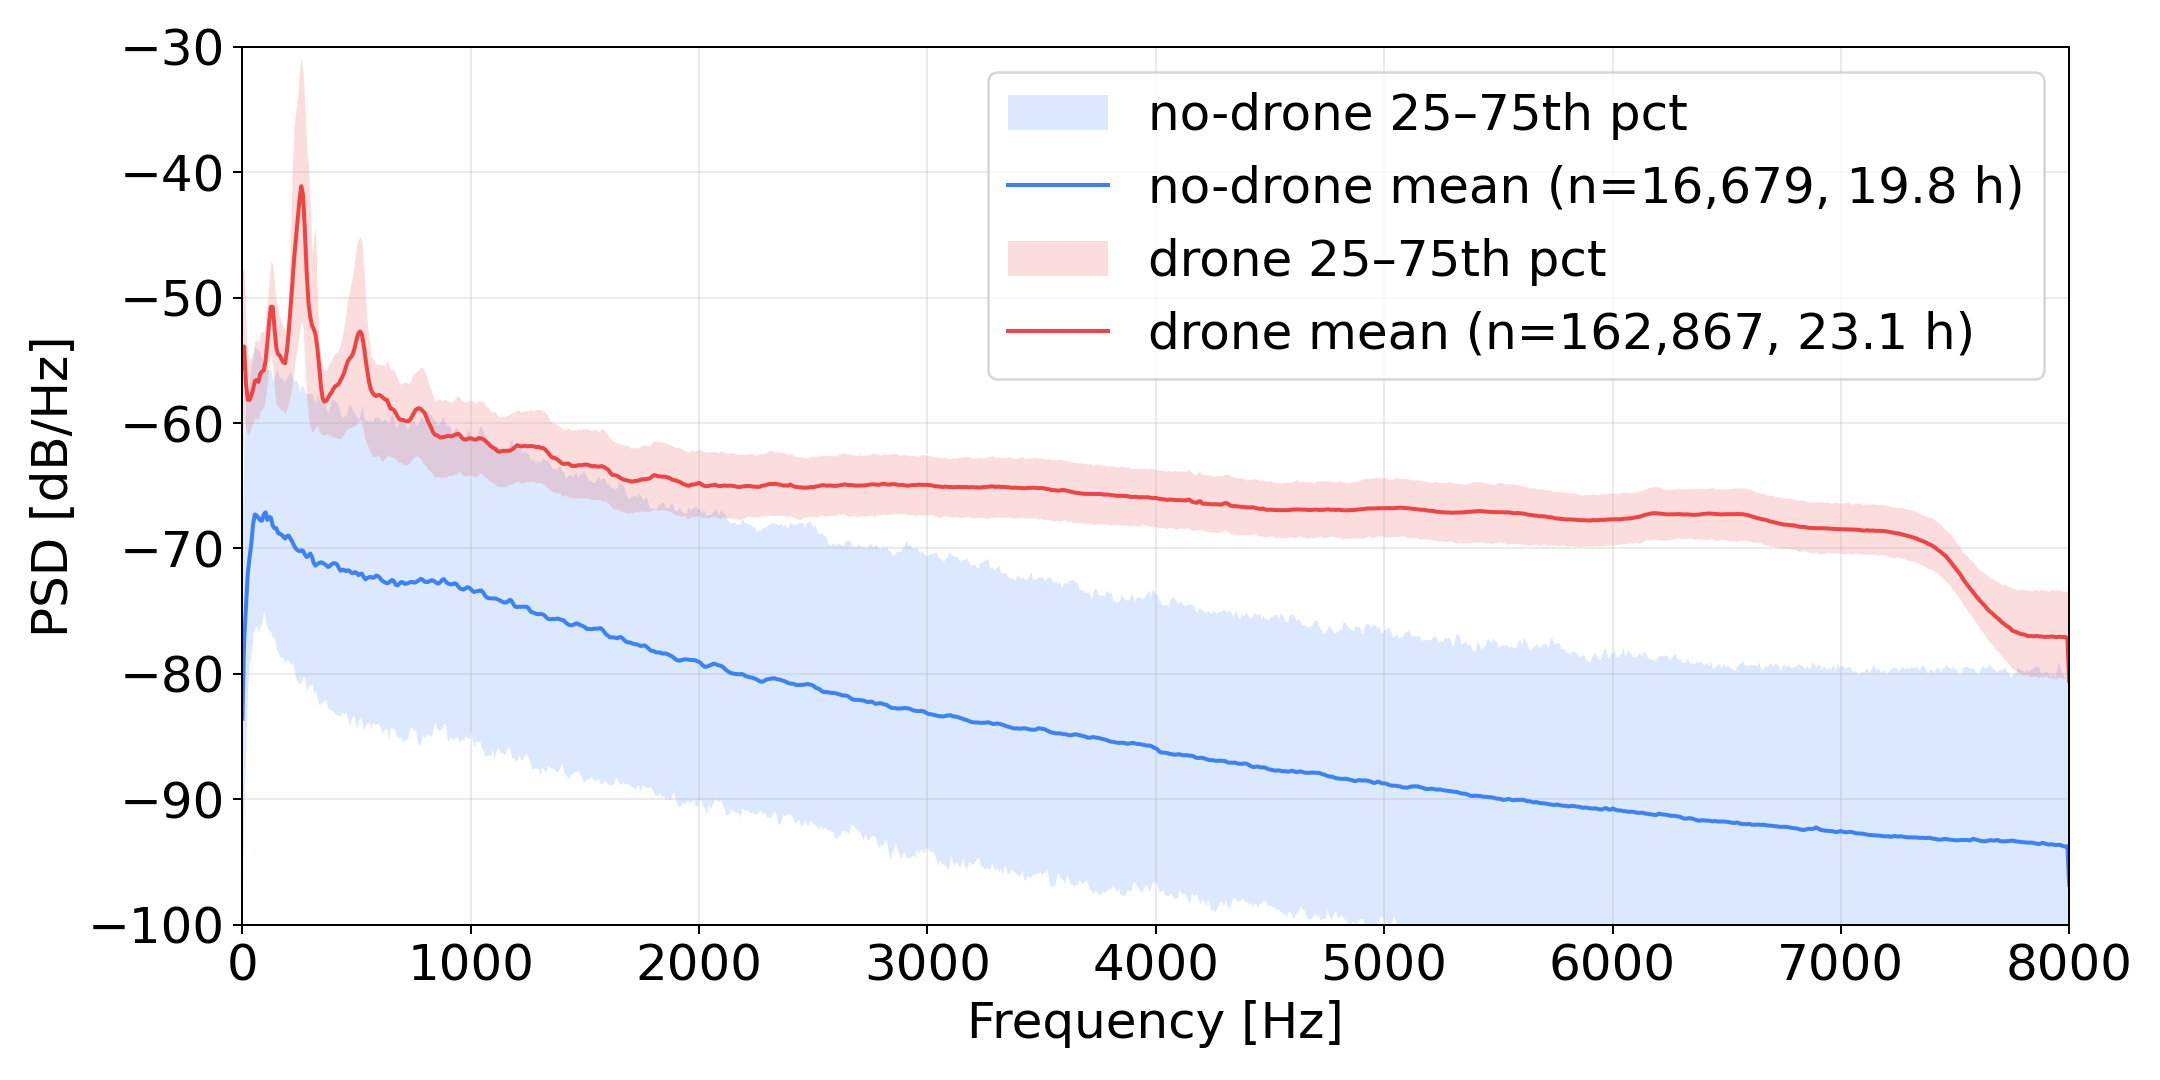
\includegraphics[width=\columnwidth]{figures/dads_average_spectrum.png}
  \caption{Střední PSD pro dronové ($n=163\,591$, červeně) a~ne-dronové ($n=14\,868$, modře) nahrávky z~datasetu DADS. Pásma odpovídají 25.–75.~percentilu přes nahrávky. Modrý region označuje ANC pracovní pásmo (0–1\,kHz).}
  \label{fig:dads_spectrum}
\end{figure}

\section{Princip FxLMS}
Základní feedforward ANC model pracuje s referencí $x[n]$, primární cestou $P(z)$ mezi zdrojem rušení a mikrofonem, adaptivním řídicím filtrem $G(z)$ a sekundární cestou $C(z)$ mezi aktuátorem a mikrofonem. Primární signál v mikrofonu zapíšeme jako

\begin{figure}[htbp]
  \centering
  \includegraphics[width=\columnwidth]{generated/fxlms_schema.pdf}
  \caption{Blokové schéma algoritmu FxLMS s modelem sekundární cesty $\hat{C}(z)$.}
  \label{fig:fxlms_schema}
\end{figure}

\begin{equation}
  d[n] = P(z)x[n] + s[n],
\end{equation}
kde $s[n]$ označuje užitečný signál. Řídicí filtr generuje
\begin{equation}
  y[n] = \sum_{i=0}^{L-1} g_i[n]x[n-i],
\end{equation}
Po průchodu sekundární cestou vznikne odrušovací složka $c_y[n] = C(z)y[n]$. Chybový signál je
\begin{equation}
  e[n] = d[n] - c_y[n].
\end{equation}

Změna vah $g_i[n]$ se v mikrofonu projeví až přes sekundární cestu. FxLMS proto v adaptační větvi nepoužívá přímo $x[n]$, ale filtrovanou referenci
\begin{equation}
  x_f[n] = \hat{C}(z)x[n],
\end{equation}
kde $\hat{C}(z)$ je odhad sekundární cesty. Aktualizace vah používá \emph{normalizovaný} krok (varianta NLMS pro FxLMS)
\begin{equation}
  g_i[n+1] = g_i[n] + \frac{\mu}{P[n]}\, e[n]\,x_f[n-i],
  \label{eq:fxlms_update}
\end{equation}
kde $\mu$ je bezrozměrná rychlost učení a $P[n]$ je okamžitý výkon filtrované reference v okně délky filtru $L$,
\begin{equation}
  P[n] = \varepsilon + \sum_{i=0}^{L-1} x_f^2[n-i].
  \label{eq:fxlms_power}
\end{equation}
Malá kladná konstanta $\varepsilon$ regularizuje jmenovatel: zabraňuje dělení nulou a~přílišnému kroku, když je reference tichá. V implementaci se tato rovnice počítá ve fixed-point aritmetice Q15 se saturací výstupu i vah.

\subsection*{Normalizovaný krok a jeho význam}
U~klasického LMS kroku $\mu\,e[n]\,x_f[n-i]$ je efektivní velikost úměrná výkonu filtrované reference. Mez stability i~rychlost konvergence proto závisejí na hlasitosti vstupu: $\mu$ vyladěné pro jednu úroveň signálu může pro jinou úroveň divergovat, nebo konvergovat příliš pomalu. Dělení výkonem $P[n]$ tuto závislost odstraňuje --- efektivní krok $\mu/P[n]$ je vůči úrovni vstupu invariantní, takže $\mu$ je bezrozměrný parametr s~prakticky stabilním rozsahem zhruba $0<\mu\lesssim 1$ (v~práci volíme $\mu\approx 0{,}5$). To je klíčové pro vícekanálovou konfiguraci: jak ukazuje následující sekce, $P[n]$ se sčítá přes \emph{všechny} reference a~aktuátory, takže stejné $\mu$ funguje pro SISO i~pro libovolný počet kanálů bez ručního přeškálování.

\subsection*{Vektorové rozšíření}

Pro více referencí a více chybových mikrofonů přecházíme na vektorový zápis (obr.~\ref{fig:fxlms_schema_multiple}). Označme $X$ počet referenčních kanálů (motorových referencí) a $M$ počet chybových mikrofonů. Referenční vektor $\mathbf{x}(n)\in\mathbb{R}^{X}$ vstupuje do maticového adaptivního filtru $\mathbf{G}(z)\in\mathbb{R}^{X\times X}$, který produkuje $X$ aktuátorových signálů. Sekundární cesta $\mathbf{C}(z)\in\mathbb{R}^{M\times X}$ mapuje výstupy aktuátorů do $M$ mikrofonů a generuje chybový vektor $\mathbf{e}(n)\in\mathbb{R}^{M}$. Odhad $\hat{\mathbf{C}}(z)$ filtruje referenci a vznikne matice filtrovaných referencí $\mathbf{x}'(n)\in\mathbb{R}^{X}$, která vstupuje do adaptační aktualizace.

V implementaci odpovídá $X$ parametru \code{--reference-count} a $M$ počtu chybových mikrofonů (v současném modelu $M=1$). Počet aktuátorů je nastaven parametrem \code{--actuator-count}; ve zjednodušeném schématu na obr.~\ref{fig:fxlms_schema_multiple} je ztotožněn s~$X$.

\begin{figure}[htbp]
  \centering
  \includegraphics[width=\columnwidth]{generated/fxlms_schema_multiple.pdf}
  \caption{Blokové schéma vektorového FxLMS pro $X$ referenčních kanálů a $M$ chybových mikrofonů. Silné šipky označují vektory; křížky na vodičích ukazují dimenzi ($X$ nebo $M$). Adaptivní filtr $\mathbf{G}(z)\in\mathbb{R}^{X\times X}$ generuje $X$ aktuátorových signálů; $\mathbf{C}(z)\in\mathbb{R}^{M\times X}$ je fyzická sekundární cesta; $\hat{\mathbf{C}}(z)$ je její odhad použitý ve filtraci reference.}
  \label{fig:fxlms_schema_multiple}
\end{figure}

\section{Implementace}
Kód je v modulu \code{scripts/lms-filter}. Python generuje syntetickou scénu, připravuje WAV soubory, volá sdílenou C knihovnu a ukládá grafy s metrikami. C jádro obsahuje fixed-point FxLMS filtr. Samotné jádro nealokuje haldu; volající předá stavový buffer o velikosti vypočtené z konfigurace. Hostitelský wrapper používá alokaci jen pro demonstrační API.

\subsection{SISO režim}
SISO varianta používá jednu referenci a jeden aktuátor. Je to základní baseline s jedním adaptivním FIR filtrem $G(z)$, jednou historií reference, jednou sekundární cestou $C(z)$ a jedním odhadem $\hat{C}(z)$.

\subsection{Sum-first a MISO režimy}
Pro více motorových referencí používáme dva režimy. V režimu \emph{sum-first} Python nejdříve sečte syntetické reference jednotlivých motorů. C jádro potom dostane jeden referenční kanál ($X=1$). Se čtyřmi aktuátory tedy běží čtyři adaptivní filtry.

V režimu \emph{MISO} (viz obr.~\ref{fig:fxlms_schema_multiple}) vstupuje do C jádra plná matice $X$ referencí. Pro $X$ referencí a $A$ aktuátorů se alokuje $A \times X$ adaptivních FIR filtrů. Konfigurace \code{--reference-count 4 --actuator-count 4} tedy vytvoří 16 sad vah ($X=4$, $A=4$, $M=1$). Výstup aktuátoru $a$ je součet příspěvků všech referencí:
\begin{equation}
  y_a[n] = \sum_{r=0}^{X-1}\sum_{i=0}^{L-1} g_{a,r,i}[n]x_r[n-i].
\end{equation}
Sekundární výstupy aktuátorů se sčítají do jedné odrušovací složky v chybovém mikrofonu ($M=1$). Všechny adaptivní cesty se učí ze stejného chybového signálu $e[n]$. Každá cesta ale používá vlastní filtrovanou referenci $x_{f,a,r}[n]=\hat{C}_a(z)x_r[n]$ přes odhad sekundární cesty daného aktuátoru a~aktualizace váhy $g_{a,r,i}$ má tvar~\eqref{eq:fxlms_update} s~$x_f$ nahrazeným za $x_{f,a,r}$.

Normalizační výkon $P[n]$ z~\eqref{eq:fxlms_power} se ve vícekanálovém případě sčítá přes \emph{všechny} dvojice reference--aktuátor,
\begin{equation}
  P[n] = \varepsilon + \sum_{a=0}^{A-1}\sum_{r=0}^{X-1}\sum_{i=0}^{L-1} x_{f,a,r}^2[n-i].
  \label{eq:fxlms_power_multi}
\end{equation}
Tím se efektivní krok automaticky zmenší úměrně počtu a~energii kanálů, takže stejné $\mu$ zůstává stabilní při růstu $X$ i~$A$. Dřívější varianta s~pevným krokem to řešila hrubým dělením $\mu$ konstantou pro vícekanálový režim; normalizace tento ad-hoc zásah nahrazuje a~odstraňuje propad útlumu, který přeškálování způsobovalo.

V C implementaci není sekundární cesta $C(z)$ odvozena z geometrie ani z měření reálného reproduktoru. Pro každý aktuátor $a$ je modelována samostatným pevným čtyřkoeficientovým FIR filtrem $C_a(z)$ v aritmetice Q15. Jeho vstupem je řídicí signál $y_a[n]$ na výstupu adaptivního filtru, tedy signál před aktuátorem, a výstup představuje odrušovací akustickou složku v místě chybového mikrofonu:
\begin{equation}
  c_a[n] = \sum_{k=0}^{3} c_{a,k}y_a[n-k].
\end{equation}
Úlohou tohoto FIR filtru je aproximovat impulzní odezvu sekundární fyzické cesty. Aktuální vzorek $y_a[n]$ a jeho tři předchozí hodnoty jsou násobeny jednotlivými koeficienty a sečteny. Výstup proto není pouze zesílenou kopií řídicího signálu: FIR filtr do něj zavádí krátkou časovou paměť, frekvenčně závislý útlum a fázový posun, které přibližují odezvu aktuátoru a šíření zvuku k mikrofonu. To je pro FxLMS podstatné, protože odrušovací signál musí dorazit do místa měření se správnou amplitudou a opačnou fází vůči primárnímu hluku. Použité čtyři koeficienty představují pouze krátký demonstrační model; věrnější model reálné sestavy by vznikl identifikací delší impulzní odezvy z měření.

Koeficienty jsou v programu uloženy v poli \code{k\_secondary\_path}; jednotlivé aktuátory používají mírně odlišné sady koeficientů, aby reprezentovaly rozdílné přenosy od aktuátoru k mikrofonu. Tento FIR filtr je pevnou součástí simulovaného prostředí a jeho koeficienty se během adaptace nemění. Tím se liší od FIR filtrů regulátoru $G(z)$, jejichž váhy algoritmus průběžně upravuje s cílem minimalizovat $e[n]$. FIR výpočet používá kruhovou historii, pořadí koeficientů od nejnovějšího vzorku a po akumulaci posun o 15 bitů se saturací. Při více aktuátorech se jejich sekundární výstupy sečtou a z jediného simulovaného mikrofonního signálu se vypočte
\begin{equation}
  e[n] = d[n] - \sum_{a=0}^{A-1} c_a[n].
\end{equation}
Blok $C_a(z)$ tak v modelu zastupuje celý přenos od elektrického výstupu regulátoru přes aktuátor a šíření zvuku až k chybovému mikrofonu; tyto fyzické části nejsou simulovány odděleně. Odhad $\hat{C}_a(z)$ je implementován dalším čtyřkoeficientovým FIR filtrem s podobnými, ale záměrně neidentickými koeficienty z pole \code{k\_secondary\_path\_estimate}. Používá se pouze k filtraci referencí pro aktualizaci vah, nikoliv k tvorbě signálu $e[n]$.

\subsection{Fixed-point aritmetika}
Veřejné vzorky a koeficienty mají typ \code{int16\_t} ve stylu Q15. FIR výpočet akumuluje v širším integer typu a výsledek posouvá o 15 bitů. Aktualizace vah podle \eqref{eq:fxlms_update} se počítá v~64bitové aritmetice: čitatel $\mu\,e[n]\,x_f[n-i]$ (parametr \code{mu\_q15} v~Q15, tj. $\mu=\code{mu\_q15}/2^{15}$) se celočíselně dělí jmenovatelem $P[n]$ a~výsledný přírůstek se přičte k~váze se saturací do rozsahu \code{int16\_t}. Výkon $P[n]$ je veden jako klouzavý součet čtverců filtrovaných referencí přes okno délky $L$ a~přes všechny kanály: při každém vzorku se odečte čtverec vzorku opouštějícího okno a~přičte čtverec nového, takže přepočet je $O(1)$ na kanál místo $O(L)$. Regularizace $\varepsilon$ je odvozena z~počtu kanálů a~délky filtru. Protože normalizace dělí krok výkonem sečteným přes všechny kanály, není potřeba žádné ruční přeškálování \code{mu\_q15} podle počtu referencí ani aktuátorů --- stejná hodnota se používá pro SISO i~vícekanálové konfigurace.

\section{Experimentální metodika}
Experimenty v této verzi používají simulaci. Python vytváří hluk dronu z více motorových referencí s různými otáčkami, gainy, zpožděními a FIR primárními cestami. Užitečný WAV signál se normalizuje, zkrátí nebo doplní na délku simulace a přičte k primárnímu mikrofonnímu signálu. Výstup FxLMS je chybový signál. V ideálním případě v něm zůstane užitečná událost a klesne složka korelovaná s motory.

Pro první sadu výsledků je připraven scénář s impulzním audio souborem \code{audio/gunshot-vs-firecracker.wav}. Referenční běh pro MISO konfiguraci je:
\begin{quote}
\scriptsize\ttfamily
task run --\\
--wanted-wav audio/gunshot-vs-firecracker.wav\\
--duration-s 10 --plot-window 5..6\\
--spectrum-window 5..6 --wanted-gain 0.1\\
--mode miso --reference-count 4\\
--actuator-count 4
\end{quote}

Hlavní metriky budou převzaty z \code{metrics.json}: MSE primárního signálu, MSE chybového signálu, MSE reziduálního dronového hluku a útlum dronu v decibelech:
\begin{equation}
  A_{\mathrm{drone}} = 10\log_{10}\frac{\mathrm{MSE}(d_{\mathrm{drone}})}{\mathrm{MSE}(e-s)}.
\end{equation}
Tato metrika není metrika detekce výstřelu. Měří pouze to, zda filtr snížil složku vlastního hluku dronu v okně, ve kterém chceme později spouštět detektor impulzních událostí.

\section{Připravená výsledková část}
Tabulka~\ref{tab:metrics_placeholder} má plánovaný tvar výsledkové tabulky. Hodnoty budou doplněny po vygenerování finálních experimentálních artefaktů.

\begin{table}[htbp]
\caption{Plánované metriky pro porovnání konfigurací}
\label{tab:metrics_placeholder}
\centering
\begin{tabular}{lccc}
\toprule
Režim & Reference & Aktuátory & Útlum dronu [dB] \\
\midrule
SISO & 1 & 1 & TBD \\
sum-first & 1 & 4 & TBD \\
MISO & 4 & 4 & TBD \\
\bottomrule
\end{tabular}
\end{table}

\begin{figure}[htbp]
\centering
\placeholder{Místo pro časový průběh: wanted, noisy input, ANC output a residual v okně 5..6 s.}
\caption{Plánovaný časový graf impulzní události před a po FxLMS filtraci.}
\label{fig:time_placeholder}
\end{figure}

\begin{figure}[htbp]
\centering
\placeholder{Místo pro PSD graf: noisy input, wanted, ANC output a frekvenční útlum dronu.}
\caption{Plánované spektrální porovnání před a po FxLMS filtraci.}
\label{fig:spectrum_placeholder}
\end{figure}

\section{Diskuze a budoucí práce}
Současný model reprezentuje akustické cesty pevnými FIR filtry a ručně zvolenými zpožděními. Neobsahuje souřadnice motorů, mikrofonů a reproduktorů, výpočet zpoždění z rychlosti zvuku, směrové charakteristiky ani odrazy. Z aktuálních výsledků proto nepůjde odvozovat prostorový beampattern ani účinnost směrového maskování zvukové stopy dronu.

Směrové maskování vyžaduje geometrický model dronu a okolního prostoru. Každý motor, reproduktor a mikrofon musí mít definovanou pozici. Primární a sekundární cesty pak mohou vznikat ze vzdálenosti, útlumu, propagation delay a jednoduchého modelu odrazů. Nad takovým modelem půjde formulovat úlohu, ve které reproduktory snižují nebo maskují akustickou stopu ve zvoleném směru a současně kontrolují energii vyzařovanou jinam.

Pro detekci impulzních událostí je další krok jednodušší: přidat detektor a změřit jeho chování před a po FxLMS filtraci. První verze může používat krátkodobou energii nebo spektrální změnu. Až poté má smysl přejít na klasifikátor.

\section{Závěr}
Text shrnul implementaci FxLMS filtru pro potlačení vlastního hluku dronu v simulovaném palubním mikrofonu. Kód podporuje SISO, sum-first a MISO režimy. Multi-channel konfigurace vytváří matici adaptivních filtrů mezi motorovými referencemi a aktuátory. Připravená metodika počítá s doplněním grafů a metrik pro scénáře s impulzním užitečným signálem. Směrové maskování zůstává oddělená navazující úloha, protože vyžaduje geometrický a akustický model prostoru.

\bibliographystyle{ieeetr}
\bibliography{references}

\end{document}
